\begin{figure}
    \centering
    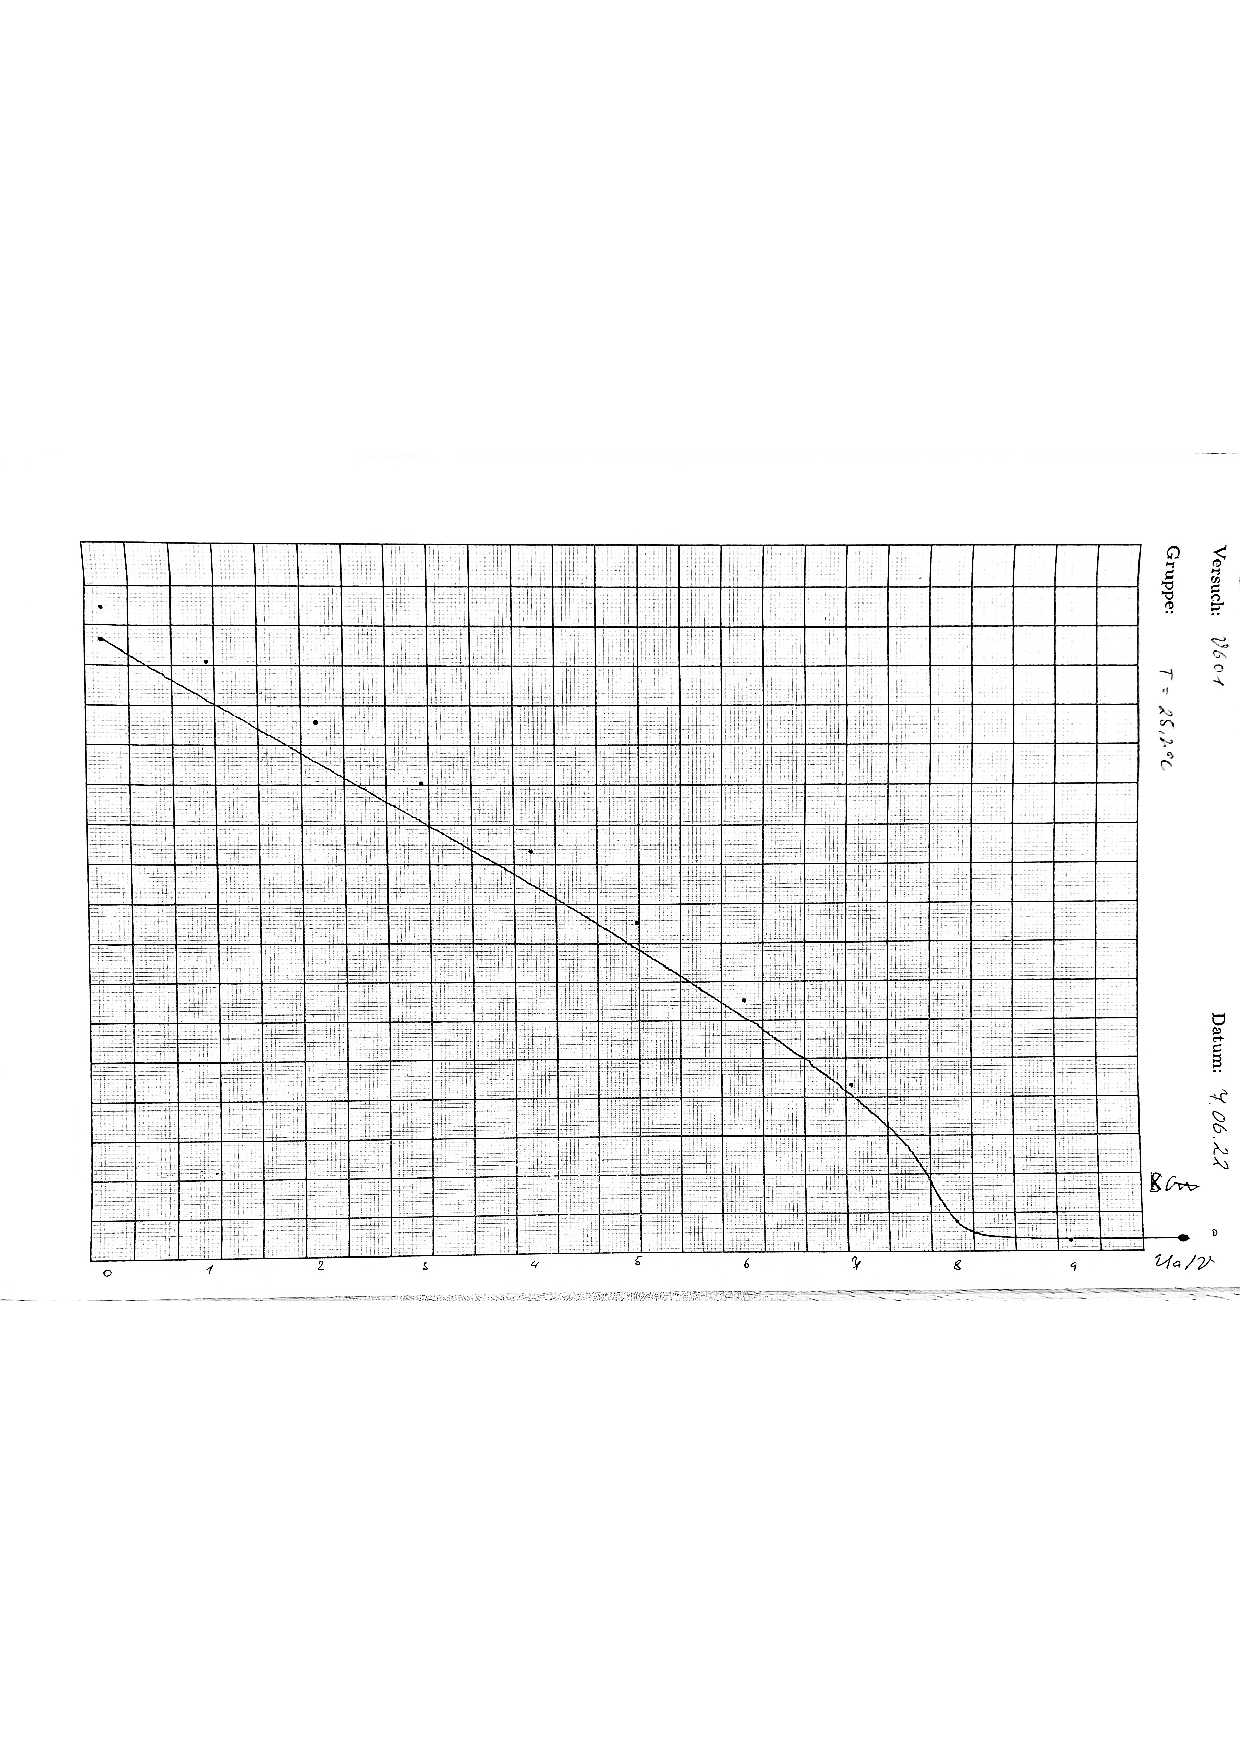
\includegraphics[width=0.8\linewidth]{pictures/kurve1.pdf}
    \caption{Die erste Messung.}
    \label{fig:kurve1}
\end{figure}

\begin{figure}
    \centering
    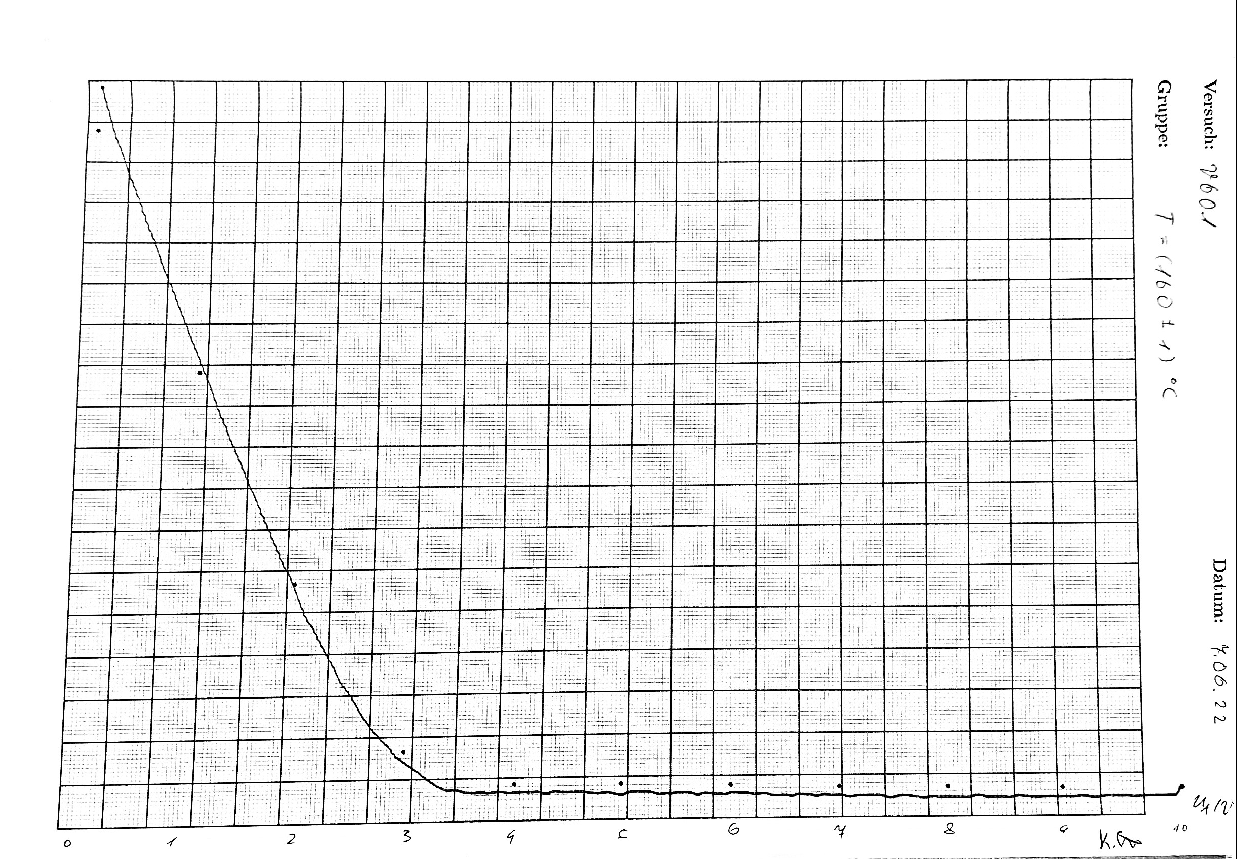
\includegraphics[width=0.8\linewidth]{pictures/kurve2_1.pdf}
    \caption{Die zweite Messung.}
    \label{fig:kurve2}
\end{figure}

\begin{figure}
    \centering
    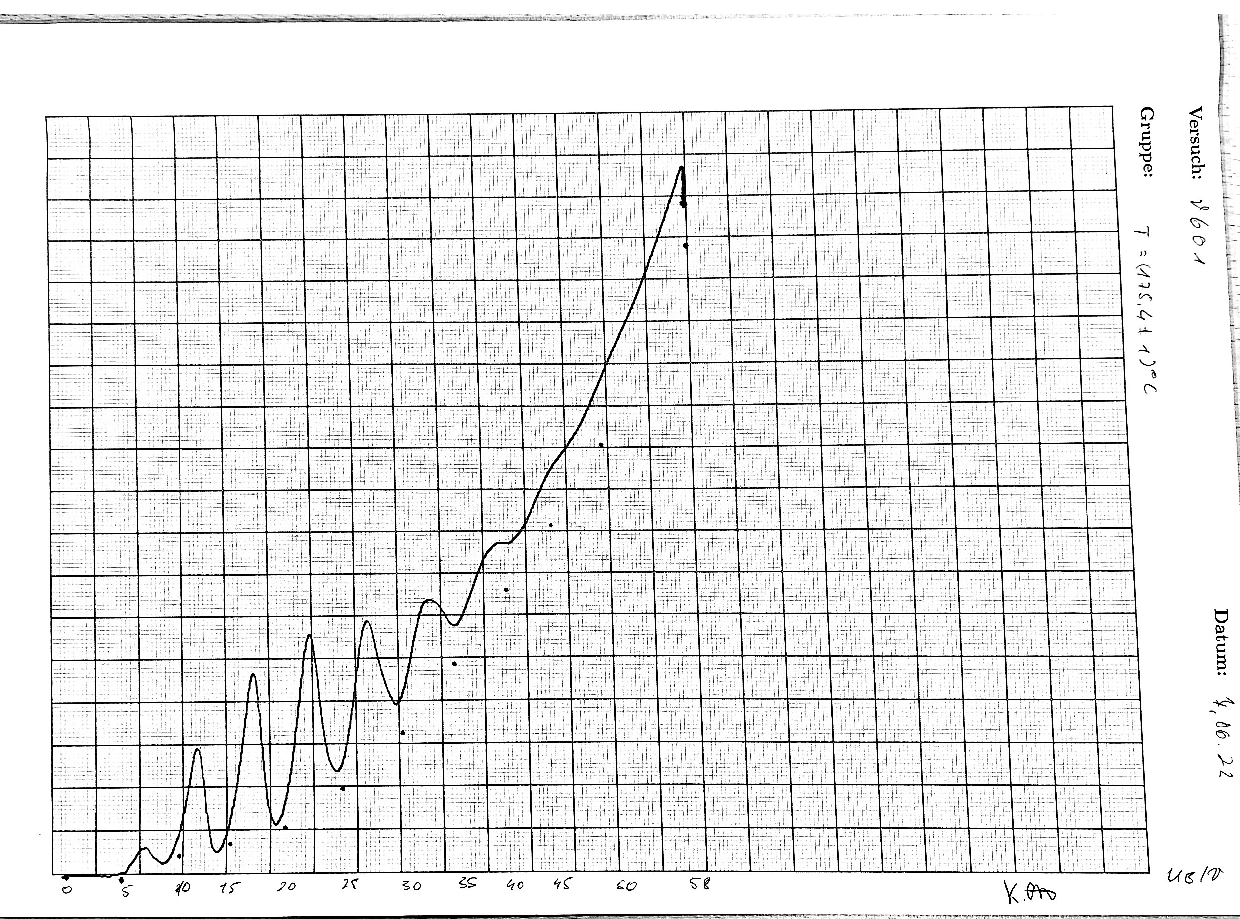
\includegraphics[width=0.8\linewidth]{pictures/kurve3.pdf}
    \caption{Die dritte Messung.}
    \label{fig:kurve3}
\end{figure}

\begin{figure}
    \centering
    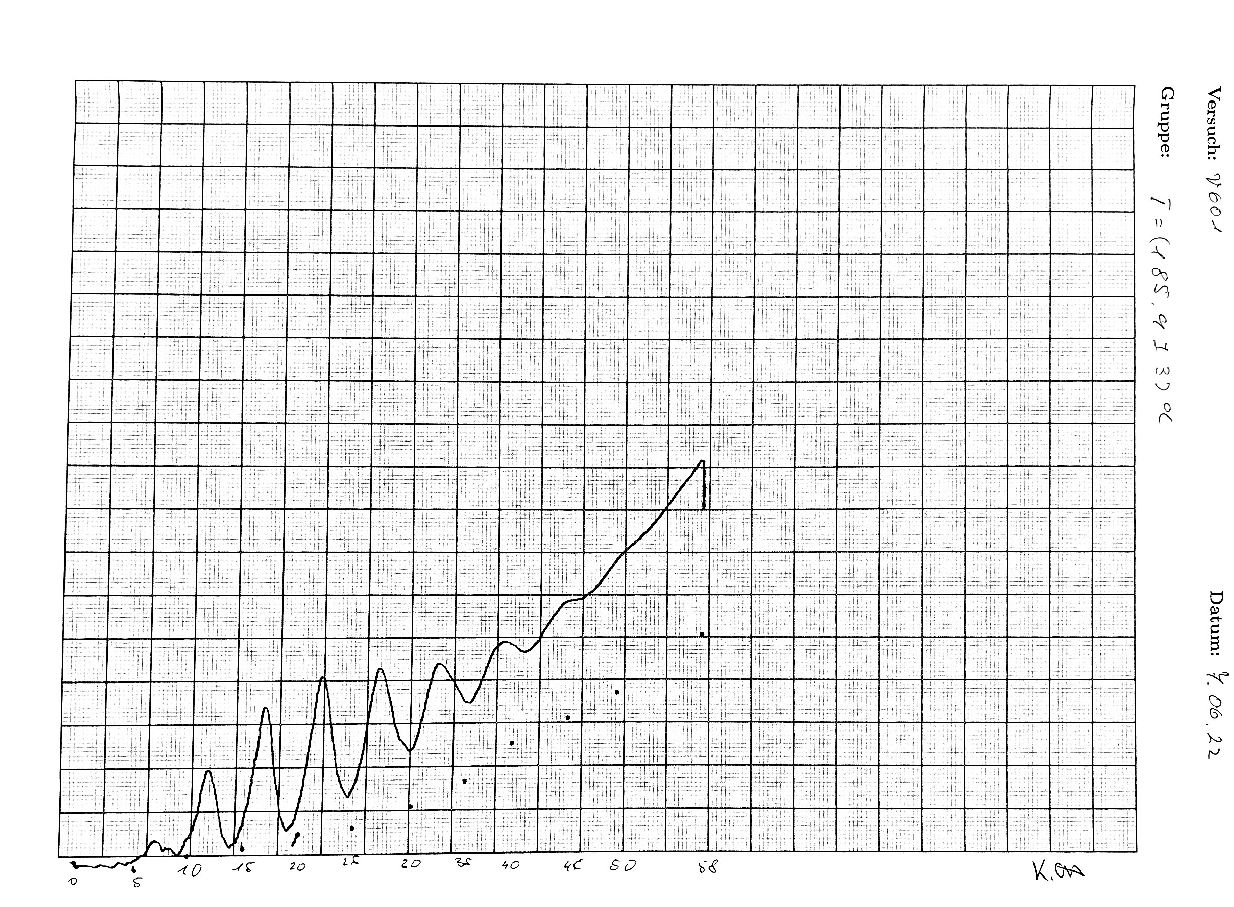
\includegraphics[width=0.8\linewidth]{pictures/kurve4.pdf}
    \caption{Die vierte Messung.}
    \label{fig:kurve4}
\end{figure}